\chapter*{付録A Raspberry Pi Cat}

\section{Raspberry Pi Cat}
Raspberry Pi Cat(以下ラズパイキャット)は図\ref{fig:raspicat}で示された二輪の差動駆動型ロボットである. 
また, ラズパイキャットは既製品の小型移動ロボットである.
このロボットについて説明をする.
\begin{figure}[h]
	\begin{center}
		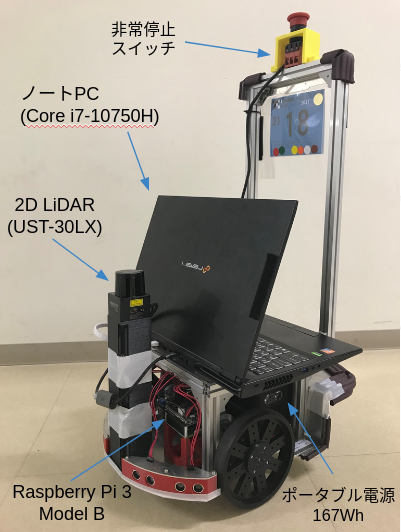
\includegraphics[width=0.5\linewidth]{figs/raspicat.png}
		\caption{}
		\label{fig:raspicat}
	\end{center}
\end{figure}

\subsection{使用したコンピュータのスペック}

\subsubsection{Raspberry Pi 3 Model B}
SoCはBroadcom BCM2837 1.2GHz×4(CPU).
メモリは1GB.
\subsubsection{ノートPC}
CPUはCore i7-10750H 2.6GHz×12. 
GPUはNVIDIA GeForce RTX 2070.
メモリは32GB.

\subsection{2D LiDAR}
使用した2D LiDARはHOKUYOのUST-30LXである.
UST-30LXの走査角度は270度, 角度分解能は0.25度, 測定分解能は1mm, 最大検出距離は60mである.

地面などのノイズを観測せずに多くのランドマークを獲得するために図\ref{fig:raspicat-lidar}
のように地面から36cmの高さに取り付けた.

\begin{figure}[h]
	\begin{center}
		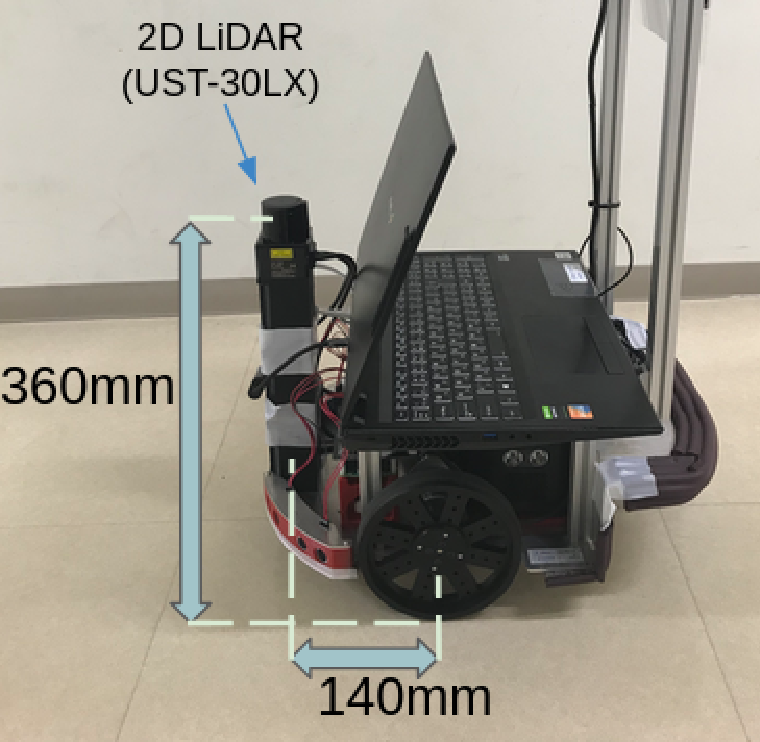
\includegraphics[width=0.5\linewidth]{figs/raspicat-lidar.pdf}
		\caption{}
		\label{fig:raspicat-lidar}
	\end{center}
\end{figure}

\subsection{ハードウェア構成}
ラズパイキャットのハードウェア構成を図\ref{fig:raspicat-hardware-config}に示す. 
搭載されている外界センサは, 2D LiDAR(UST-30LX)のみである.この2D LiDARのみで
自己位置推定や障害物回避を実現している. 
モータの速度制御としてRaspberry Pi 3 Model Bが搭載されており, モータは
Raspberry Pi 3 Model Bから送られてくる速度指令値に基づいてモータドライバによって駆動されている.

自己位置推定や行動計画のための計算機としてノートPC(Intel i7-10750H)を搭載している.
また, Raspberry Pi 3 Model BとノートPCはLANケーブルによる接続で通信を行っている.

\begin{figure}[h]
	\begin{center}
		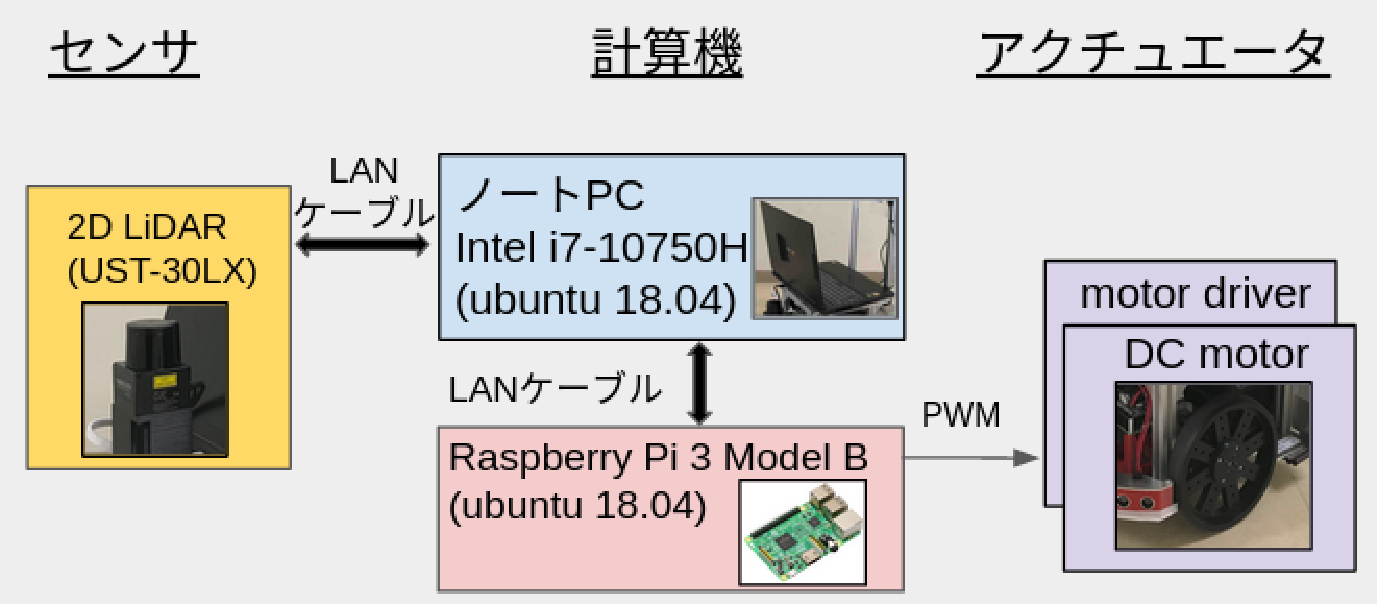
\includegraphics[width=1.0\linewidth]{figs/raspicat-hardware-config.pdf}
		\caption{}
		\label{fig:raspicat-hardware-config}
	\end{center}
\end{figure}

\subsection{ソフトウェア構成}
ラズパイキャットのソフトウェア構成を図\ref{fig:raspicat-software-config}に示す.
ラズパイキャットはロボットの制御システムとしてROSを使用している.Raspberry Pi 3 Model Bではmotorsノードのみが立ち上がっており, 
モータの制御を行っている. 
ノートPCでは, amclやmove\_base等のノードが立ち上がっており, 
自己位置推定や行動計画を行っている.

オドメトリにはimuなどは使用しておらず, 
motorsノードで速度指令値(/cmd\_vel)を積算させたデッドレコニング(/odom)を使用している. 
そのため, 急回転には弱いが非常に簡素なシステムになっているためシステムの
立ち上げミスが少ない.



\begin{figure}[H]
	\begin{center}
		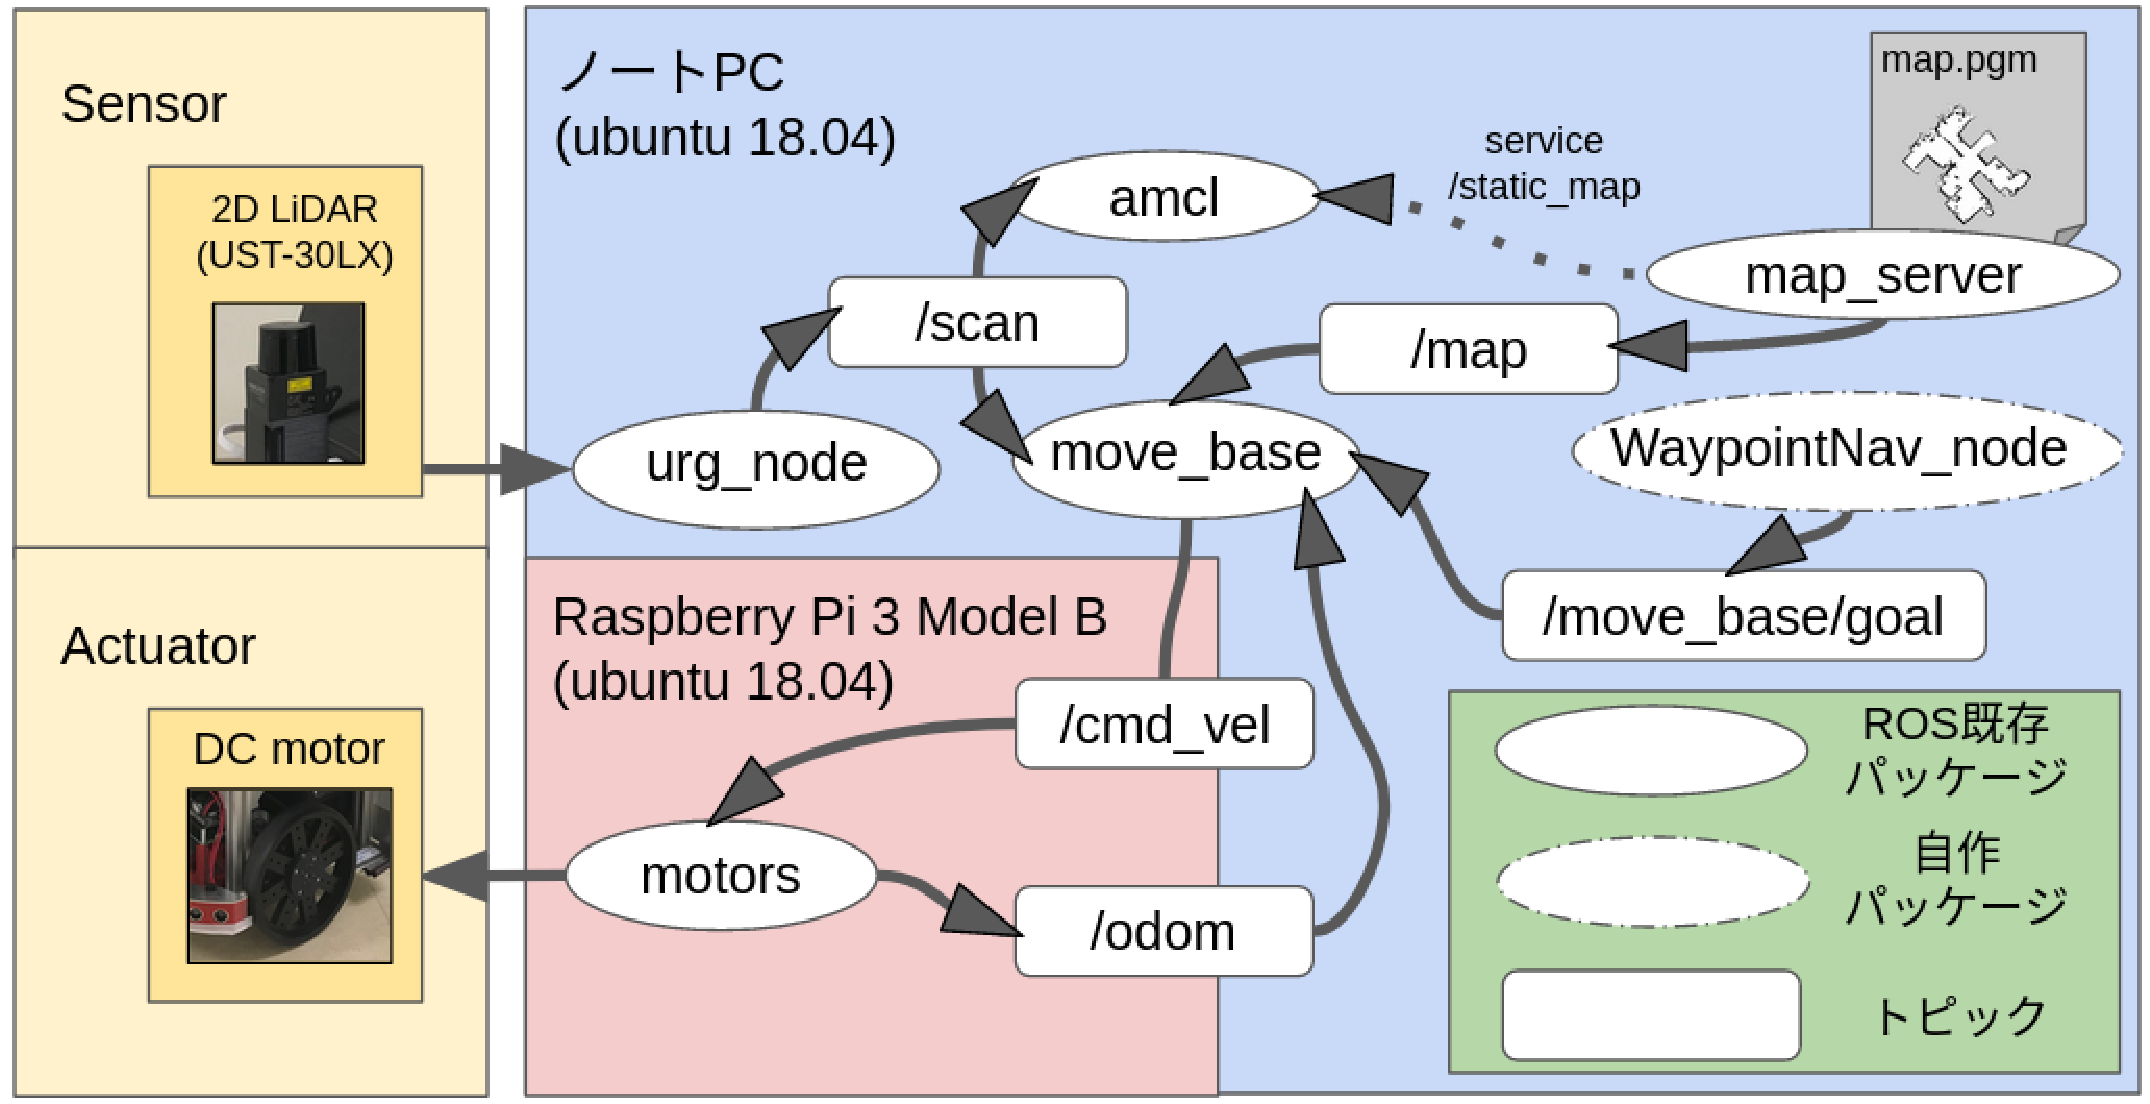
\includegraphics[width=0.9\linewidth]{figs/raspicat-software-config.pdf}
		\caption{}
		\label{fig:raspicat-software-config}
	\end{center}
\end{figure}